\pagebreak
\subsection{Umgang mit der Karte}

	Navigation mit der Karte \\

	Die in Arma 3 verwendete topographische Karte ist sehr nützlich um geeignete Landezonen, Overwatchpositionen, Deckungsmöglichkeiten und Antrittswege im Voraus zu erkennen. Wichtig ist, dass hierbei die Höhenlinien und Symbole auf der Karte richtig interpretiert werden. Je enger die Höhenlinien, desto Steiler das Gelände. \\

 

	Hier als Beispiel von einem relativ schmalen Tal, das nach Norden, Westen und Süden von Bergen umgeben ist. \\
\begin{minipage}[t]{1\textwidth}
	\centering
	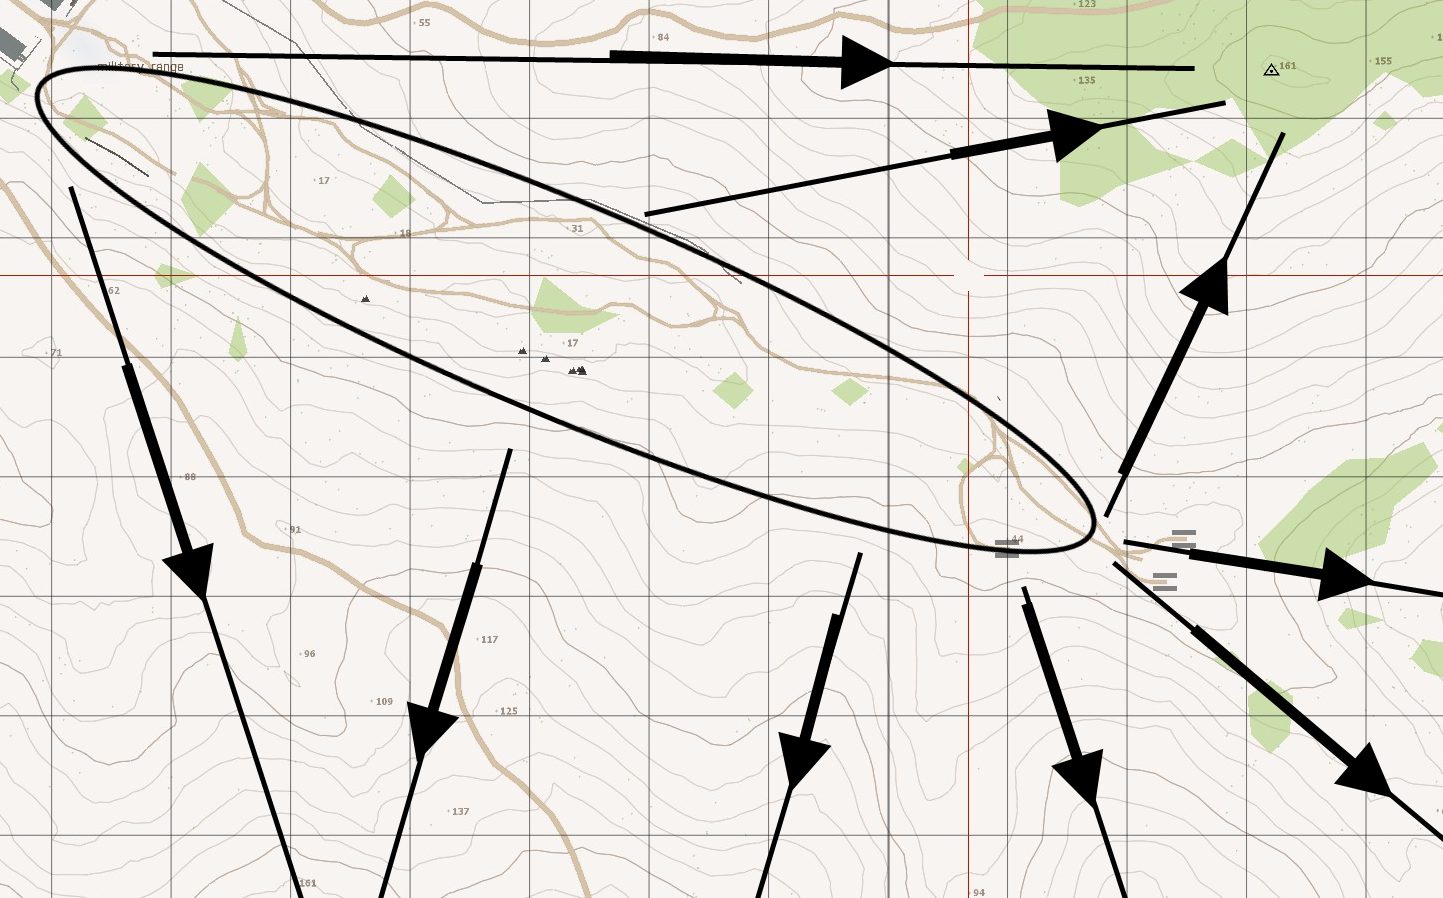
\includegraphics[width=\textwidth]{./img/fortgeschrittenes/karteUndMarkierungen/Karte1.png}
\end{minipage}

	Markante Linien sind, je nach Zoomstufe im Abstand von 1 bis 25m zueinander, beginnend mit der Wasserlinie 0 m. Berggipfel werden mit einem Dreieck mit Punkt in der Mitte dargestellt, andere Hügel mit Zahlen (Meterangabe). Oft nutzt man diese auch zur Kommunkation >>Hill 68<< ist dann zB. der 68 m Hohe Hügel im entsprechenden Planquadrat. \\

\begin{minipage}[t]{1\textwidth}
	\centering
	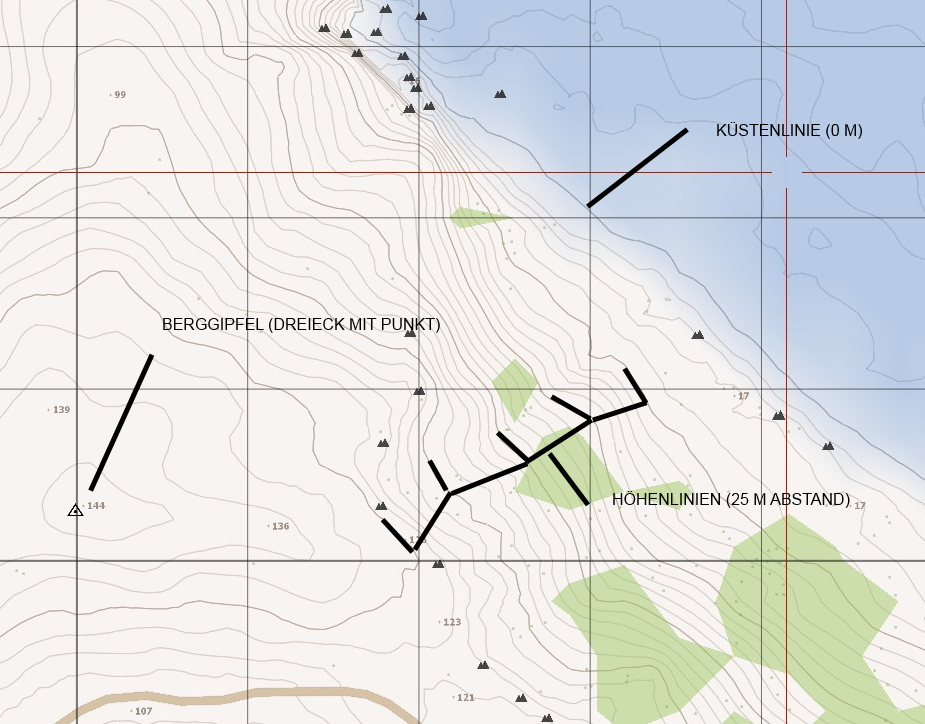
\includegraphics[width=\textwidth]{./img/fortgeschrittenes/karteUndMarkierungen/Karte2.png}
\end{minipage}

	Kartenkoordinaten werden in der Kartenansicht immer unter eurem Cursor angezeigt. Falls euch welche gegeben werden, kann dies auf zwei Wege erfolgen: „Position xxx-yyy“ oder „Planquadrat xx-yy“. Die erste Zahlenfolge bezeichnet immer die Koordinatenspalten und die zweite Zahlenfolge die Koordinatenreihen. X ist die obere, horizontale Achse, Y ist die linke, senkrechte Achse. \\

	Die Karte selbst lässt sich fliessend per Mausrad Zoomen, die Gitternetzlinien sind in der weitesten Zoomstufe in 1km Abständen, sobald man näher heranzoomt ändern sich diese zu 100 m Abständen. So lassen sich auch Feindpositionen bzw. Distanzen zu diesen besser abschätzen. \\

	Die diagonale Distanz der 100 m Kästchen sind ca. 140 m. \\

\begin{minipage}[t]{1\textwidth}
	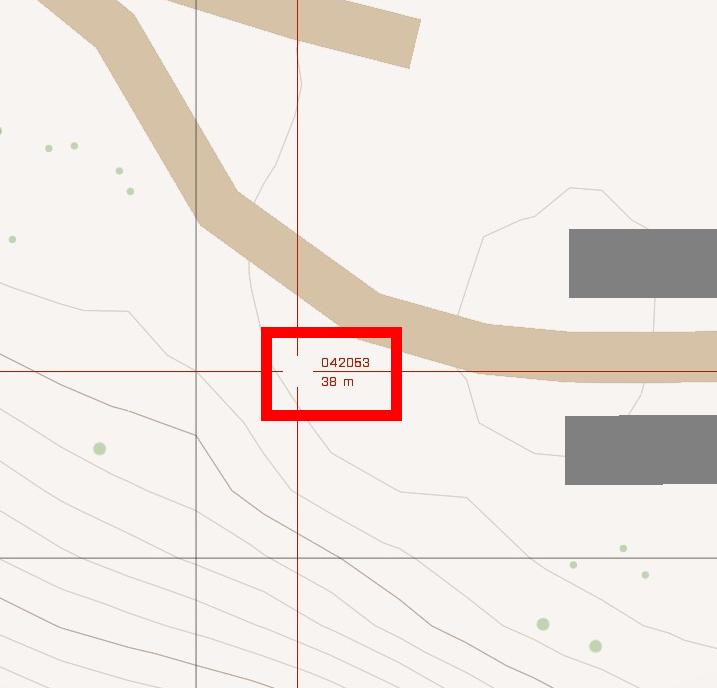
\includegraphics[width=\textwidth]{./img/fortgeschrittenes/karteUndMarkierungen/Karte3.png}
\end{minipage}

	Diese Koordinaten werden auch auf eurem GPS oben links angezeigt, so lässt sich eure Position immer genau bestimmen, falls verlangt wird, dass ihr eure eigene Position markiert bzw. um festzulegen wo Feinde zu markieren sind. \\

\begin{minipage}[t]{1\textwidth}
	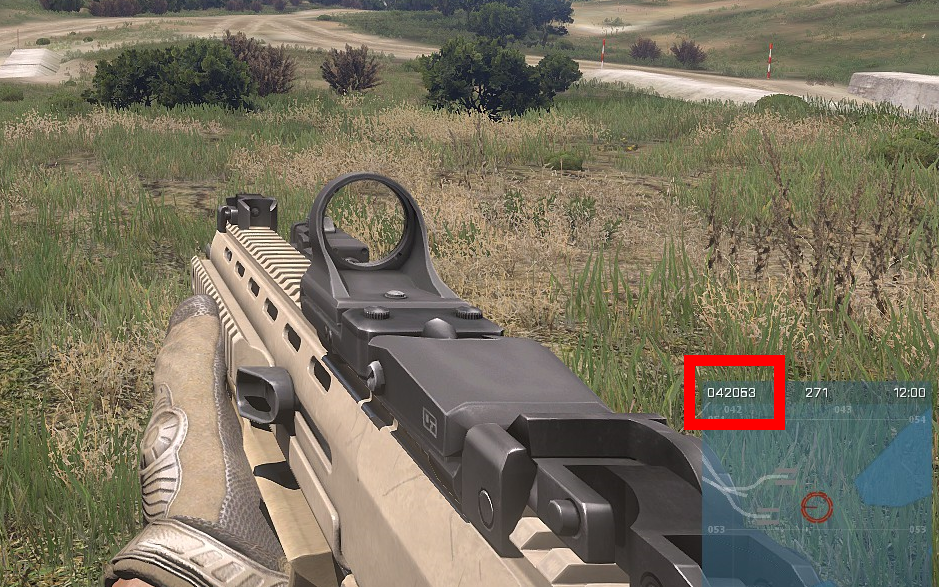
\includegraphics[width=\textwidth]{./img/fortgeschrittenes/karteUndMarkierungen/Karte4.png}
\end{minipage}